% A small KAN of shape [2, 2, 1] for the KAN subsection of Section 2.1: each edge carries a
% learnable curve (drawn as a small plot) and each node adds what reaches it.
% Compile on its own (pdflatex kan-diagram.tex); the thesis includes the PDF.
\documentclass[12pt,border=2pt]{standalone}
\usepackage[T1]{fontenc}
\usepackage{mathpazo}
\usepackage{tikz}
\usetikzlibrary{arrows.meta}
\begin{document}
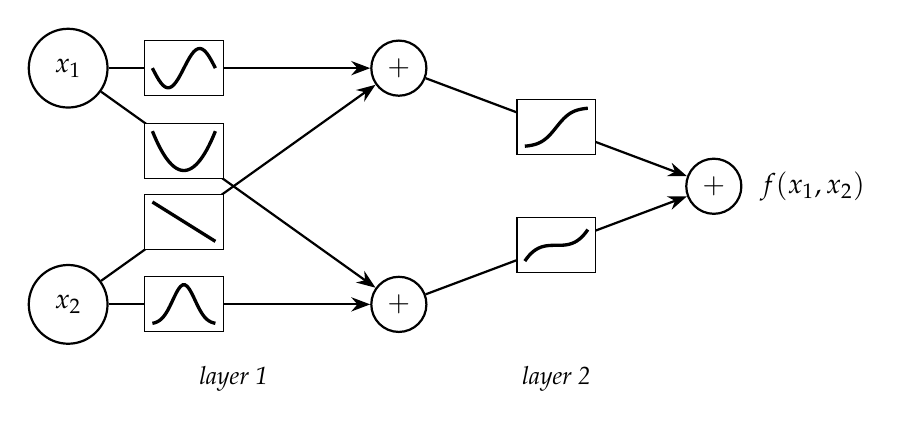
\begin{tikzpicture}[
    var/.style  = {circle, draw, thick, minimum size=10mm, inner sep=0pt},
    sum/.style  = {circle, draw, thick, minimum size=7mm, inner sep=0pt},
    arr/.style  = {-{Stealth[length=2.4mm]}, thick},
    curvebox/.style = {draw, fill=white, minimum width=10mm, minimum height=7mm, inner sep=0pt},
    word/.style = {font=\small\itshape}
  ]
  % \curveat{centre}{expression in \x for x in [-1, 1], output roughly in [-1, 1]}
  \newcommand{\curveat}[2]{%
    \node[curvebox] at #1 {};
    \begin{scope}[shift={#1}, x=0.4cm, y=0.25cm]
      \draw[very thick, domain=-1:1, samples=30] plot (\x, {#2});
    \end{scope}}

  \node[var] (X1) at (0,  1.5) {$x_1$};
  \node[var] (X2) at (0, -1.5) {$x_2$};
  \node[sum] (H1) at (4.2,  1.5) {$+$};
  \node[sum] (H2) at (4.2, -1.5) {$+$};
  \node[sum] (O)  at (8.2,  0)   {$+$};
  \node[right=1mm] at (O.east) {$f(x_1, x_2)$};

  \draw[arr] (X1) -- (H1);
  \draw[arr] (X1) -- (H2);
  \draw[arr] (X2) -- (H1);
  \draw[arr] (X2) -- (H2);
  \draw[arr] (H1) -- (O);
  \draw[arr] (H2) -- (O);

  % first layer: boxes at 35% of each edge, so that the crossing edges keep their boxes apart
  \curveat{(1.47,  1.5)}{sin(180*\x)}
  \curveat{(1.47,  0.45)}{\x*\x*2 - 1}
  \curveat{(1.47, -0.45)}{-\x}
  \curveat{(1.47, -1.5)}{2*exp(-4*\x*\x) - 1}
  % second layer: boxes at the middle of each edge
  \curveat{(6.2,  0.75)}{tanh(2*\x)}
  \curveat{(6.2, -0.75)}{0.8*\x*\x*\x}

  \node[word] at (2.1, -2.45) {layer 1};
  \node[word] at (6.2, -2.45) {layer 2};
\end{tikzpicture}
\end{document}
